\section{APPENDICES}

\subsection{Time Plan}
% \textbf{Time plan}

\begin{table}[H]
  \begin{center}
    \leavevmode
\hangcaption[Semester 1 Time-plan]{Semester 1 Time-plan}
\begin{tabular}{|l|c|c|c|c|c|c|c|c|c|c|c|} \hline
& \multicolumn{11}{c|}{SEMESTER 1} \\ \hline
\rowcolor{white} Week & 1 & 2 & 3 & 4 & 5 & 6 & 7 & 8 & 9 & 10 & 11 \\ \hline
\rowcolor{white} Project Proposal & & \cellcolor{black} & \cellcolor{black} & \cellcolor{black} & & & & & & & \\ \hline
\rowcolor{white} Continuous Presentation & & & & & \cellcolor{black} & \cellcolor{black} & \cellcolor{black} & \cellcolor{black} & \cellcolor{black} & \cellcolor{black} & \cellcolor{black} \\ \hline
\rowcolor{white} Literature Review & & & & & & \cellcolor{black} & \cellcolor{black} & \cellcolor{black} & \cellcolor{black} & \cellcolor{black} & \cellcolor{black} \\ \hline
\rowcolor{white} Mechanical Design & & & & & & & \cellcolor{black} & \cellcolor{black} & \cellcolor{black} & \cellcolor{black} & \\ \hline
\rowcolor{white} Electrical Design & & & & & & & \cellcolor{black} & \cellcolor{black} & \cellcolor{black} & \cellcolor{black} & \\ \hline
\rowcolor{white} Software Design & & & & & & & & & \cellcolor{black} & \cellcolor{black} & \cellcolor{black} \\ \hline
\rowcolor{white} Material Acquisition & & & & & & & & & & & \cellcolor{black} \\ \hline
\end{tabular}
\label{table:semester1timeplan}
\end{center}
\end{table}

\begin{table}[H]
  \begin{center}
    \leavevmode
\hangcaption[Semester 2 Time-plan]{Semester 2 Time-plan}
\begin{tabular}{|l|c|c|c|c|c|c|c|c|c|c|c|c|c|c|} \hline
& \multicolumn{14}{c|}{SEMESTER 2} \\ \hline
\rowcolor{white} Week & 1 & 2 & 3 & 4 & 5 & 6 & 7 & 8 & 9 & 10 & 11 & 12 & 13 & 14 \\ \hline
\rowcolor{white} Continuous Presentation & \cellcolor{black} & \cellcolor{black} & \cellcolor{black} & \cellcolor{black} & \cellcolor{black} & \cellcolor{black} & \cellcolor{black} & \cellcolor{black} & \cellcolor{black} & & & & & \\ \hline
\rowcolor{white} Literature Review & \cellcolor{black} & \cellcolor{black} & \cellcolor{black} & \cellcolor{black} & \cellcolor{black} & & & & & & & & & \\ \hline
\rowcolor{white} Material Acquisition & \cellcolor{black} & \cellcolor{black} & & & & & & & & & & & & \\ \hline
\rowcolor{white} Mechanical Fabrication & & \cellcolor{black} & \cellcolor{black} & \cellcolor{black} & \cellcolor{black} & & & & & & & & & \\ \hline
\rowcolor{white} Electrical Fabrication & & & \cellcolor{black} & \cellcolor{black} & \cellcolor{black} & \cellcolor{black} & & & & & & & & \\ \hline
\rowcolor{white} Software Fabrication & & & & \cellcolor{black} & \cellcolor{black} & \cellcolor{black} & \cellcolor{black} & \cellcolor{black} & \cellcolor{black} & & & & & \\ \hline

\rowcolor{white} Assembly & & & & & & \cellcolor{black} & \cellcolor{black} & \cellcolor{black} & \cellcolor{black} & \cellcolor{black} & & & & \\ \hline
\rowcolor{white} Testing & & & & & & \cellcolor{black} & \cellcolor{black} & \cellcolor{black} & \cellcolor{black} & \cellcolor{black} & \cellcolor{black} & \cellcolor{black} & & \\ \hline
\rowcolor{white} Demonstration & & & & & & & & & & \cellcolor{black} & \cellcolor{black} & \cellcolor{black} & \cellcolor{black} & \cellcolor{black} \\ \hline
\end{tabular}

\label{table:semester2timeplan}
\end{center}
\end{table}

\subsection{Budget}
\begin{table}[H]
  \begin{center}
    \leavevmode
    \hangcaption[Cost Budget]{Cost Budget}
     \begin{tabular}{| l | c | c | c | c | c |}\hline
No. & Item & Quantity & Supplier & Unit Cost & Total cost \\\hline
1 & Satima S2 Motor driver & 4 & Pixel Electric & 500 & 2000 \\\hline
2 & STM32F103C8T6 & 1 & Nerokas & 1000 & 1000 \\\hline
3 & MPU-6050 & 1 & Nerokas & 260 & 260 \\\hline
4 & Esp 12 F & 2 & Nerokas & 300 & 600 \\\hline
5 & Passive components & 1 & Pixel Electric & 1000 & 1000 \\\hline
6 & PCB & 2 & & 500 & 1000 \\\hline
7 & 18650 Lithium Ion Battery & 5 & Pixel Electric & 350 & 1750 \\\hline
8 & DC motor & 8 & Pixel Electric & 1100 & 8800 \\\hline
9 & Motor Bracket & 8 & Pixel Electric & 300 & 2400 \\\hline
10 & Motor shaft and couplings & 4 & Pixel Electric & 200 & 800 \\\hline
11 & Bearing & 4 & Hardware & 100 & 400 \\\hline
12 & V-belt pulley & 16 & Pixel Electric & 150 & 2400 \\\hline
13 & Belt & 8 & Hardware & 200 & 1600 \\\hline
14 & Castor Wheels & 4 & Nerokas & 200 & 800 \\\hline
15 & Steel rods & 5 & Hardware & 60 & 300 \\\hline
16 & Aluminium Sheet & 1 & Hardware & 600 & 600 \\\hline
17 & Fasteners & 1 & Hardware & 500 & 500 \\\hline
18 & Miscalleneous & 1 & & 2600 & 2600 \\\hline
& & & & & \\\hline
& & & & TOTAL & 28810 \\\hline
    \end{tabular}
    \label{table:1}
  \end{center}
\end{table}


\begin{table}[H]
  \begin{center}
    \leavevmode
    \hangcaption[Power Budget]{Power Budget}
     \begin{tabular}{| l | c | c | c | c |}\hline
Component & Voltage (V) & Current (mA) & No. of Components & Power (W) \\\hline
MPU6050 & 3.3 & 4.68 & 1 & 0.015444 \\\hline
ESp32 & 3.3 & 480 & 1 & 1.584 \\\hline
Stm32 & 3.3 & 360 & 1 & 1.188 \\\hline
Led & 3.3 & 120 & 2 & 0.792 \\\hline
DC motor & 12 & 360 & 4 & 34.56 \\\hline
Stepper motor & 12 & 450 & 2 & 10.8 \\\hline
Motor driver & 5 & 43.2 & 1 & 0.216 \\\hline
& & & & 49.155444 \\\hline
    \end{tabular}
    \label{table:1}
  \end{center}
\end{table}

\subsection{PCB Designs}

\begin{figure}[H]
    \centering
    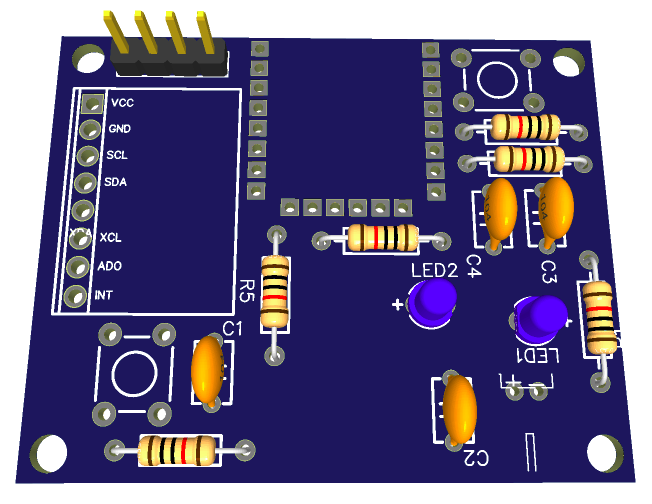
\includegraphics[scale=0.5]{Figures/HMpcb_top.png}
    \caption{Hand Motion Top view of PCB}
    \label{fig:handmotiontopview}
\end{figure}


\begin{figure}[H]
    \centering
    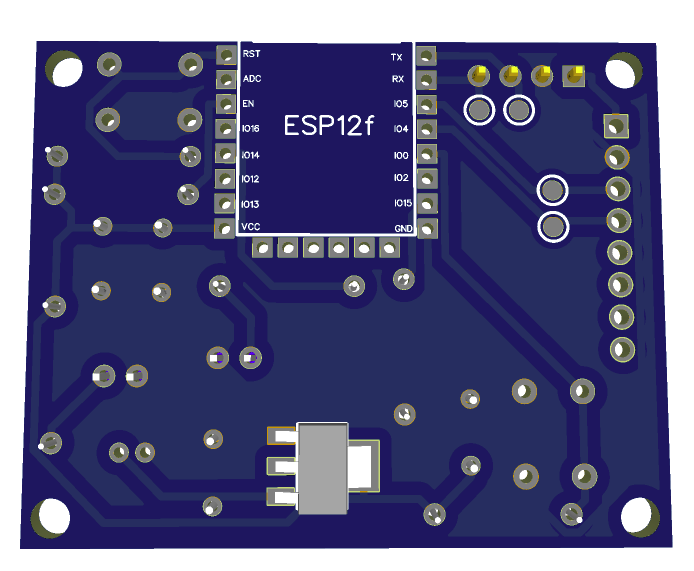
\includegraphics[scale=0.5]{Figures/HMpcb_bottom.png}
    \caption{Hand Motion Bottom view of PCB}
    \label{fig:handmotionbottomview}
\end{figure}

% TODO - Add Hand Motion Fabricated Design

\begin{figure}[H]
    \centering
    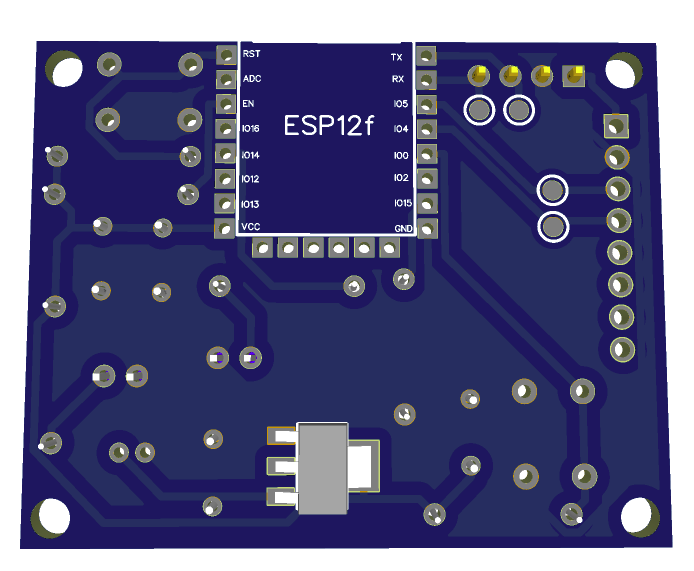
\includegraphics[scale=0.5]{Figures/HMpcb_bottom.png}
    \caption{Hand Motion Fabricated PCB}
    \label{fig:handmotionfabricatedpcb}
\end{figure}

\begin{figure}[H]
    \centering
    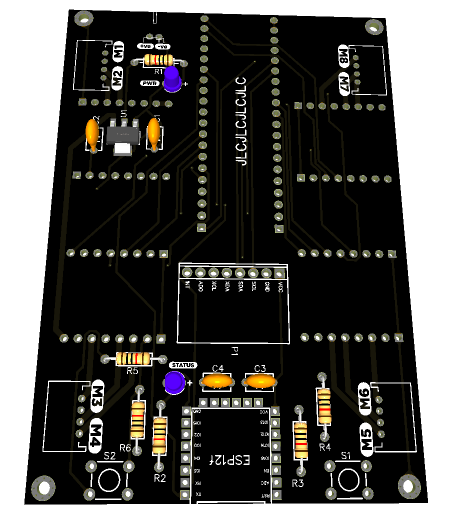
\includegraphics[scale=0.5]{Figures/MPpcb_top.png}
    \caption{Mobile Platform top view}
    \label{fig:mobileplatformtopview}
\end{figure}

\begin{figure}[H]
    \centering
    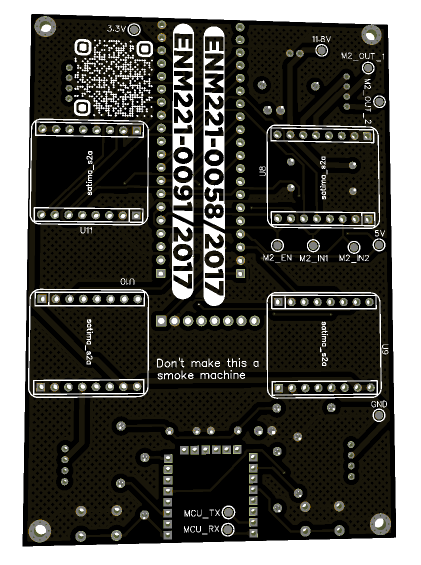
\includegraphics[scale=0.5]{Figures/MPpcb_bottom.png}
    \caption{Mobile Platform bottom view}
    \label{fig:mobileplatformbottomview}
\end{figure}

% TODO - Add Mobile Platform Fabricated Design

\begin{figure}[H]
    \centering
    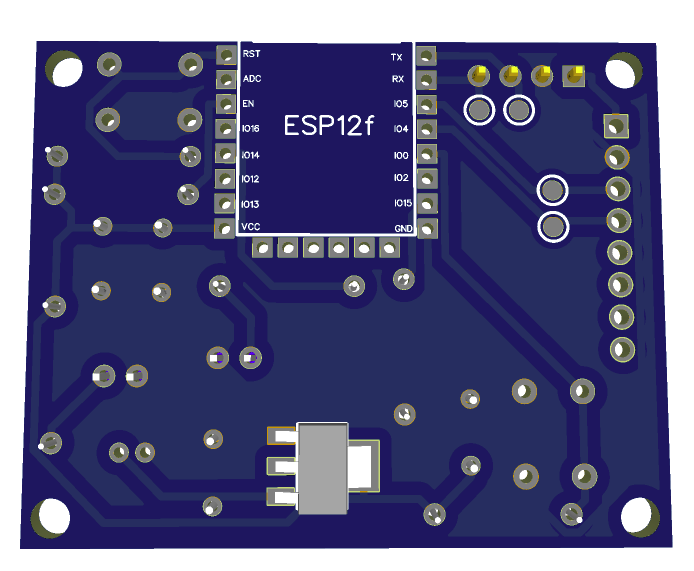
\includegraphics[scale=0.5]{Figures/HMpcb_bottom.png}
    \caption{Mobile Platform Fabricated PCB}
    \label{fig:mobileplatformfabricatedpcb}
\end{figure}

\subsection{PCB Manual Fabrication Process}
\label{sec:PCBfab}
\begin{enumerate}
    \item Print out the bottom layer onto the shiny side of the glossy paper. The copper pads and tracks should be black
    \item Sand the copper plate so there is a rough surface for the design to stick to when transferred
    \item Wash the copper with some water and rubbing alcohol and let it dry
    \item Cut out the designs and place them face down on the copper
    \item Run the copper plate with the design face down through a laminator or iron box 5-7 times until the plate is hot
    \item After running the plate through a laminator or iron place the plate into a cold bath and agitate until the paper floats of
    \item Place the PCB into the etching solution and agitate for 25-30 minutes or until all the copper has dissolved around the design
    \item Once all the copper is gone rinse it in the water bath, let it dry and use rubbing alcohol to whip off the ink transferred onto the PCB
    \item Drill the holes for DIP components and also mounting holes
    \item Start by placing SMD components and solder them either by hot air gun or hand soldering
    \item Solder DIP components by hand soldering
\end{enumerate}


\subsection{Production Plan}
% Please add the following required packages to your document preamble:
% \usepackage{graphicx}
\begin{table}[H]
\centering
\caption{Production plan}
\label{tab:productionPlan}
\resizebox{\textwidth}{!}{%
\begin{tabular}{|clllll|}
\hline
\multicolumn{6}{|c|}{\textbf{Production Plan}} \\ \hline
\multicolumn{1}{|c|}{\textbf{Week}} &
  \multicolumn{1}{l|}{\textbf{Tasks/Activities}} &
  \multicolumn{1}{c|}{\textbf{Material Required}} &
  \multicolumn{1}{c|}{\textbf{Special Equipment}} &
  \multicolumn{1}{c|}{\textbf{Concurrent Activities}} &
  \multicolumn{1}{c|}{\textbf{Remarks}} \\ \hline
\multicolumn{1}{|c|}{\textbf{1}} &
  \multicolumn{1}{l|}{Presentation} &
  \multicolumn{1}{l|}{N/A} &
  \multicolumn{1}{l|}{N/A} &
  \multicolumn{1}{l|}{N/A} &
  Done \\ \hline
\multicolumn{1}{|c|}{2} &
  \multicolumn{1}{l|}{\begin{tabular}[c]{@{}l@{}}-Project production feasibility test \\ with Technician\\ -Material Acquisition \\ -Hand Motion PCB etching process\\ -Mobile Platform PCB delivery \\ and testing\end{tabular}} &
  \multicolumn{1}{l|}{Copper clad} &
  \multicolumn{1}{l|}{N/A} &
  \multicolumn{1}{l|}{Mobile App UI development} &
  Completed \\ \hline
\multicolumn{1}{|c|}{\textbf{3}} &
  \multicolumn{1}{l|}{\begin{tabular}[c]{@{}l@{}}Mechanical Fabrication commences \\ for both the body and chassis.\\ - Metal sheet cutting for the body\\ - Metal sheet folding for the body \\ and wheel shell\\ - Metal Sheet drilling for the chassis\end{tabular}} &
  \multicolumn{1}{l|}{\begin{tabular}[c]{@{}l@{}}Glalvanised Iron \\ Sheet Metal\end{tabular}} &
  \multicolumn{1}{l|}{\begin{tabular}[c]{@{}l@{}}- Drill bits\\ - Drilling Machining\\ - Hack saw\end{tabular}} &
  \multicolumn{1}{l|}{\begin{tabular}[c]{@{}l@{}}Mobile App development\\ Procure electrical components \\ and mechanical parts \\ for power transmission\end{tabular}} &
  \begin{tabular}[c]{@{}l@{}}Primary Activities \\ Done\\ \\ \\ \\ Concurrent Activities \\ Done\end{tabular} \\ \hline
\multicolumn{1}{|c|}{4} &
  \multicolumn{1}{l|}{\begin{tabular}[c]{@{}l@{}}Mechanical Assembly of the \\ different parts:\\ - Join wheel shell to the top shaft\\ - Join the chassis to each other\\ - Join chassis to outframe\\ - Assemble the body with the chassis\end{tabular}} &
  \multicolumn{1}{l|}{\begin{tabular}[c]{@{}l@{}}Mild Steel Rod\\ Nuts and Bolts\end{tabular}} &
  \multicolumn{1}{l|}{\begin{tabular}[c]{@{}l@{}}Gas WeldingMIG \\ Welding\end{tabular}} &
  \multicolumn{1}{l|}{\begin{tabular}[c]{@{}l@{}}Assemble Mobile Platform PCB\\ Drive motors using motor driver \\ and test workability\\ Clean parts from rust\end{tabular}} &
  \begin{tabular}[c]{@{}l@{}}Primary Activities \\ Done\\ \\ \\ \\ Concurrent Activities \\ Done\end{tabular} \\ \hline
\multicolumn{1}{|c|}{\textbf{5}} &
  \multicolumn{1}{l|}{\begin{tabular}[c]{@{}l@{}}Electrical Tests:\\ - Drive the motors independently\\ - Get gesture signals from hand \\ motion controller\end{tabular}} &
  \multicolumn{1}{l|}{\begin{tabular}[c]{@{}l@{}}-DC motors \\ -Stepper Motor\\ -Fully Assembled\\  Hand Motion Controller\\ -Assembled Mobile Platform\end{tabular}} &
  \multicolumn{1}{l|}{\begin{tabular}[c]{@{}l@{}}Oscilloscope\\ Multimeter\\ Signal generator\end{tabular}} &
  \multicolumn{1}{l|}{\begin{tabular}[c]{@{}l@{}}Backend Application (Build)\\ - Send message using MQTT \\ and receive it using MQTT and \\ vice  versa\\ - Send message using Web Socket \\ and Receive using MQTT and vice \\ versa\\ - Send message using HTTP and \\ receive it using MQTT and vice \\ versa\end{tabular}} &
  \begin{tabular}[c]{@{}l@{}}Primary Activities \\ Done\\ \\ \\ \\ Concurrent Activities \\ Done\end{tabular} \\ \hline
\multicolumn{1}{|c|}{6} &
  \multicolumn{1}{l|}{\begin{tabular}[c]{@{}l@{}}Assemble the motors to the platform \\ together with the transmission system\end{tabular}} &
  \multicolumn{1}{l|}{N/A} &
  \multicolumn{1}{l|}{N/A} &
  \multicolumn{1}{l|}{Backend Application Deploy} &
  \begin{tabular}[c]{@{}l@{}}Primary Activities \\ Done\\ \\ Concurrent Activities \\ Done\end{tabular} \\ \hline
\multicolumn{1}{|c|}{\textbf{7}} &
  \multicolumn{1}{l|}{\begin{tabular}[c]{@{}l@{}}- Write Mobile Platform Code\\  for holonomic and omnidirectional \\  motions\\ - Drive the Mobile Platform with\\  static code inside the Microcontroller\end{tabular}} &
  \multicolumn{1}{l|}{N/A} &
  \multicolumn{1}{l|}{N/A} &
  \multicolumn{1}{l|}{Mobile App development} &
  \begin{tabular}[c]{@{}l@{}}Primary Activities \\ Done\\ \\ Concurrent Activities \\ Done\end{tabular} \\ \hline
\multicolumn{1}{|c|}{8} &
  \multicolumn{1}{l|}{\begin{tabular}[c]{@{}l@{}}Drive the Mobile Platform using \\ Mobile Applications\end{tabular}} &
  \multicolumn{1}{l|}{N/A} &
  \multicolumn{1}{l|}{N/A} &
  \multicolumn{1}{l|}{N/A} &
   \\ \hline
\multicolumn{1}{|c|}{9} &
  \multicolumn{1}{l|}{\begin{tabular}[c]{@{}l@{}}Drive the Mobile Platform using \\ Hand Motion Controller\end{tabular}} &
  \multicolumn{1}{l|}{N/A} &
  \multicolumn{1}{l|}{N/A} &
  \multicolumn{1}{l|}{\begin{tabular}[c]{@{}l@{}}Drive the Mobile Platform using \\ Mobile Applications\end{tabular}} &
   \\ \hline
\multicolumn{1}{|c|}{\textbf{10}} &
  \multicolumn{1}{l|}{Paint the Mobile Platform} &
  \multicolumn{1}{l|}{Paint} &
  \multicolumn{1}{l|}{Spray painter} &
  \multicolumn{1}{l|}{\begin{tabular}[c]{@{}l@{}}Package the PCBs and \\ Production Code to maintain \\ industry standards\end{tabular}} &
   \\ \hline
\multicolumn{1}{|c|}{11} &
  \multicolumn{1}{l|}{\begin{tabular}[c]{@{}l@{}}Drive the Platform continuously \\ to increase durability\end{tabular}} &
  \multicolumn{1}{l|}{N/A} &
  \multicolumn{1}{l|}{N/A} &
  \multicolumn{1}{l|}{\begin{tabular}[c]{@{}l@{}}Conference talk at DroidCon \\ Regarding our Project\end{tabular}} &
   \\ \hline
\multicolumn{1}{|c|}{\textbf{12}} &
  \multicolumn{1}{l|}{\begin{tabular}[c]{@{}l@{}}Drive the Platform continuously \\ to increase durability\end{tabular}} &
  \multicolumn{1}{l|}{N/A} &
  \multicolumn{1}{l|}{N/A} &
  \multicolumn{1}{l|}{Tech Expo presentations} &
   \\ \hline
\end{tabular}%
}
\end{table}

\subsection{Production Code}
\label{sec:code}

\subsubsection{Mobile Platform}

The code we developed for this research is a complex and innovative solution that leverages advanced algorithms and data structures to achieve accurate and efficient results. It has been carefully documented and tested, and it can be found here \cite{B1ackd0t_Gitu_Naibei_2022}. This includes the mobileplatform code which is responsible for driving the platform, wificlient code responsible to receiving MQTT data from WiFi and the hand motion controller.

\subsubsection{Flutter}
The flutter code is quite lengthy and complex and can be found here 
 \cite{B1ackd0t_Gitu_2022}.